\documentclass[runningheads]{llncs}
\usepackage{graphicx}
\usepackage{booktabs}
\usepackage{amsmath}
\usepackage{url}

\begin{document}

\title{Efficient Vision Transformers Match Larger Models on Cervical Cytology Classification, But In-Distribution Accuracy Does Not Predict Domain-Shift Robustness}
\titlerunning{Efficient ViTs Match Larger Models But Miss Domain-Shift Robustness}

\author{Anonymous Author(s)}
\authorrunning{Anonymous Author(s)}
\institute{Submitted for double-blind review}

\maketitle

\begin{abstract}
Lightweight vision transformers are frequently proposed for medical image
classification on the premise that they trade a small, bounded amount of
accuracy for a large reduction in compute cost, and are rarely tested for
whether that same efficiency holds under the distribution shift a deployed
model will actually encounter across clinics, scanners, and populations.
We benchmark 12 models spanning CNN, full-size vision transformer, and
efficient-vision-transformer families on cervical cytology classification
(SIPaKMeD, 5 Bethesda-relevant cytomorphology classes), then evaluate the
same models zero-shot, with no retraining or recalibration, on three
independent external cytology datasets (Herlev, Mendeley LBC, and
APCEM-Enhanced Cervical Cytology) after harmonizing all four onto a shared
binary normal/abnormal label. Contrary to the usual efficiency-accuracy
trade-off framing, the two most parameter-efficient models in the entire
registry (EfficientViT-M0 and -B0, $\sim$2.1M parameters each) are also the
two best-performing in distribution, beating every full-size baseline by
1--3 points of balanced accuracy. Under domain shift, however,
in-distribution accuracy actively misleads: EfficientViT-M0 -- the overall
in-distribution winner -- is the worst-performing model of all 12 on both
Herlev and Mendeley LBC, dropping below the chance floor on Mendeley LBC
(0.4731 balanced accuracy on a binary task), while a much larger CNN
baseline (ResNet-50) that is not the best in-distribution model on any
dataset is the most robust model on that same shift -- yet on the third,
independently sourced shift dataset (APCEM), ResNet-50 is instead the
single worst-performing model of all 12 (AUROC 0.293), while a different
CNN (MobileNetV2) becomes the only model of the 12 to clear chance
(0.6158 balanced accuracy, AUROC 0.6528). Across Mendeley LBC, CNN-family
models cluster at 0.539--0.667 balanced accuracy while eight of nine
transformer-family models cluster at 0.293--0.523 (with one transformer
landing 0.003 above the lowest CNN -- a real, reported exception, not a
clean partition); on APCEM this apparent CNN-vs-transformer split
collapses entirely, since the CNN family alone spans both the best
(MobileNetV2) and one of the worst (ResNet-50) models in the registry.
One model (MobileViT-S) collapses to a Mendeley LBC AUROC of 0.215 --
actively anti-correlated with ground truth, not merely uninformative --
while its own architectural successor (MobileViTv2) shows no such failure
and is in fact the strongest model on that milder shift condition. No
single static property we measured -- parameter count, FLOPs,
in-distribution accuracy, or architecture family/lineage -- reliably
predicts which model fails safely under domain shift, and which model
fails safely is itself not stable across which external dataset is used
to test it.

\keywords{Cervical cytology \and Vision transformers \and Domain shift \and Model efficiency \and Trustworthy medical AI}
\end{abstract}

\section{Introduction}

Cervical cancer remains substantially more curable when caught at a
localized stage, yet screening access is documented to be uneven across
rural and urban U.S. counties, and a growing literature proposes vision
transformers -- often marketed as ``efficient'' or ``lightweight''
variants -- as classification backbones for automated cytology screening.
Two questions are almost never asked together in that literature: does
the claimed efficiency actually cost accuracy on this specific task, and
does whatever backbone wins an in-distribution benchmark remain
trustworthy when the input distribution shifts, as it inevitably will
across institutions, scanners, staining protocols, and patient
populations? This paper answers both, using a single consistent benchmark
across a 12-model registry spanning three architecture families (standard
CNNs, full-size vision transformers, and efficient/mobile-oriented vision
transformers), evaluated first in distribution and then zero-shot on
three independent external cytology datasets.

Our contributions are fourfold. First, a 12-model efficiency/accuracy
benchmark on cervical cytology classification showing that, on this task,
the most parameter-efficient models in the registry are also the most
accurate -- efficiency costs nothing here, contrary to the usual framing.
Second, a systematic escalation from a 2-model to a 4-model to a full
12-model cross-dataset domain-shift evaluation on Herlev and Mendeley LBC,
each stage refining rather than simply confirming the prior stage's
finding, converging on: no single static model property predicts shift
robustness, and the in-distribution winner is the shift-robustness loser.
Third, a specific, load-bearing counterexample to ``architecture family
predicts behavior'' reasoning: MobileViT-S collapses to below-chance,
actively anti-correlated predictions on one external dataset, while its
direct architectural successor, MobileViTv2, shows no such failure and is
the single best-performing model in the registry on the other external
dataset. Fourth, a full 12-model replication of the domain-shift
evaluation on a third, independently sourced external dataset (APCEM),
which does not merely confirm the first two shifts' conclusion but
overturns the CNN-family robustness pattern they suggested: the CNN family
on APCEM contains both the single best-performing model in the entire
registry (MobileNetV2) and one of the single worst (ResNet-50), directly
falsifying any reading of the Herlev/Mendeley results as ``CNNs are the
safe family.''

\section{Related Work}

\subsection{Efficient vision transformers}

Efficiency-oriented vision transformer variants form three loose lineages
relevant to the registry benchmarked here. Hybrid local--global designs
(MobileViT \cite{mehta2022mobilevit}, MobileViTv2
\cite{mehta2022mobilevitv2}) interleave convolutional stages with
transformer blocks to keep early-stage compute cheap while retaining
global attention at coarser resolutions. Distillation-oriented designs
(DeiT \cite{touvron2021deit}) instead keep a standard ViT backbone but use
a distillation token and teacher network to reach competitive accuracy at
far smaller pretraining-data budgets than the original ViT
\cite{dosovitskiy2021vit} required. Hardware-aware designs (LeViT
\cite{graham2021levit}, TinyViT \cite{wu2022tinyvit}) reintroduce
convolutional stages specifically to improve real-device latency, not
just FLOP count, by favoring operations that map efficiently onto
standard inference kernels. EfficientViT-M0 and EfficientViT-B0, the two
smallest and most accurate models in this study, are frequently assumed to
share a lineage because timm's tag naming groups them together --
verified directly rather than assumed, they do not. EfficientViT-M0 uses
cascaded group attention \cite{liu2023efficientvit}, a Microsoft-authored
design that reduces redundant computation across attention heads by
feeding each head a different split of the input feature map.
EfficientViT-B0 belongs to an entirely unrelated MIT-authored lineage
built around multi-scale linear attention for high-resolution dense
prediction \cite{cai2023efficientvit}, originally designed for
segmentation and detection rather than classification efficiency. That
this study's two best-performing, most-efficient models come from two
architecturally unrelated papers sharing only a name is itself a small
caution against treating ``the EfficientViT family'' as one coherent
design lineage in future efficiency claims. None
of these efficiency-oriented design papers evaluate cross-institution
domain shift as part of their own efficiency claim -- efficiency and
robustness are treated as separate, unrelated properties in the
architecture literature this registry draws from, which is precisely the
gap this paper's joint evaluation addresses.

\subsection{Domain shift and model selection in medical imaging}

A substantial general (not cervical-cytology-specific) medical-imaging
literature documents that models selected on held-out in-distribution
data can degrade sharply under real-world distribution shift across
scanners, sites, and populations, motivating external-validation
practices increasingly required by regulators and journals alike.
However, this literature typically evaluates one or a small number of
architectures rather than a systematic sweep across CNN, full-size
transformer, and efficient-transformer families at matched task and
data scale, which is what distinguishes this paper's 12-model, two-shift-
dataset design: the question is not whether shift degrades performance
(well established) but \emph{whether any measurable static property of a
model predicts which model degrades least}, tested directly rather than
assumed from a single architecture's behavior.

\subsection{Adjacent cervical and oral cancer imaging work}

Adjacent recent work on cervical and oral cancer imaging includes hybrid
CNN--transformer explainability models, ensemble methods combining
calibration with post-hoc explanation, and conformal-prediction
approaches to cervical screening uncertainty, none of which jointly
evaluate efficiency and real (not synthetic) cross-institution domain
shift together -- including a stacking-ensemble cervical cancer diagnosis
approach combined with explainable AI \cite{mohiuddin2025}, which this
paper differs from by focusing on efficiency--robustness trade-offs across
a full architecture-family registry rather than a single ensemble model.

\section{Methods}

\subsection{Model registry}

Twelve models spanning three families: CNN baselines (ResNet-50
\cite{he2016resnet}, MobileNetV2 \cite{sandler2018mobilenetv2},
EfficientNet-Lite0 \cite{tan2019efficientnet}), full-size vision
transformers (ViT-Small \cite{dosovitskiy2021vit}, Swin-Tiny
\cite{liu2021swin}), and efficient/mobile-oriented vision transformers
(DeiT-Tiny \cite{touvron2021deit}, LeViT-128 \cite{graham2021levit},
TinyViT-5M \cite{wu2022tinyvit}, MobileViT-S \cite{mehta2022mobilevit},
MobileViTv2 \cite{mehta2022mobilevitv2}, EfficientViT-B0
\cite{cai2023efficientvit}, EfficientViT-M0 \cite{liu2023efficientvit}).
All timm tags verified against the pinned timm version rather than assumed
from memory; the two EfficientViT variants' source papers were confirmed
independently against timm's own model cards rather than assumed from the
shared tag prefix (see Section~2.1).

\subsection{Training and in-distribution evaluation}

All 12 models trained on SIPaKMeD \cite{plissiti2018sipakmed}
(4,049 native-resolution single-cell crops derived directly from the
dataset's own cytoplasm-polygon boundary annotations, not a pre-resized
third-party mirror), 60/15/10/15 train/val/calibration/test split, seed 13,
full 30-epoch budget with early stopping (patience 7), on a single GPU.
Reported: balanced accuracy, macro F1, AUROC, parameter count, and
measured (not estimated) inference latency.

\subsection{Cross-dataset domain-shift evaluation}

Each model evaluated zero-shot -- no retraining, no recalibration -- on
Herlev \cite{jantzen2005herlev} and Mendeley LBC
\cite{hussain2020mendeley} after harmonizing all three datasets' differing
label taxonomies onto one shared binary normal/abnormal label. This tests
generalization under the conditions this application will actually face:
different institutions, scanners, and staining protocols, not a synthetic
corruption of the same source images.

A third, independently sourced external dataset -- the APCEM-Enhanced
Cervical Cytology Pap Smear Image Dataset \cite{aswini2026apcem}, 4,253
images across the 6-class Bethesda taxonomy (NILM, ASC-US, ASC-H, LSIL,
HSIL, SSC) -- is evaluated identically, harmonized to the same binary label
(NILM normal; all five atypical/dysplastic classes abnormal). This dataset
differs from Herlev and Mendeley LBC in acquisition pipeline, institution,
and label granularity, so it functions as a genuinely independent
replication of the domain-shift evaluation rather than a second look at
the same shift.

\section{Results}

\subsection{Efficiency/accuracy benchmark}

\begin{table}[htbp]
\centering
\caption{RQ1 efficiency/accuracy benchmark, all 12 models, sorted by balanced accuracy.}
\label{tab:rq1}
\begin{tabular}{lrrrrr}
\toprule
Model & Bal.\ acc. & Macro F1 & AUROC & Params & Latency (ms) \\
\midrule
\textbf{EfficientViT-M0} & \textbf{0.9654} & \textbf{0.9656} & 0.9985 & \textbf{2{,}157{,}401} & 17.56 \\
EfficientViT-B0 & 0.9623 & 0.9624 & 0.9983 & 2{,}135{,}413 & 6.97 \\
DeiT-Tiny & 0.9606 & 0.9607 & 0.9974 & 5{,}525{,}381 & 5.17 \\
Swin-Tiny & 0.9605 & 0.9606 & 0.9965 & 27{,}523{,}199 & 11.36 \\
TinyViT-5M & 0.9587 & 0.9589 & 0.9979 & 5{,}073{,}369 & 9.57 \\
MobileViT-S & 0.9570 & 0.9575 & 0.9979 & 4{,}940{,}837 & 9.32 \\
ResNet-50 & 0.9542 & 0.9540 & 0.9966 & 23{,}518{,}277 & 5.95 \\
LeViT-128 & 0.9458 & 0.9456 & 0.9946 & 8{,}447{,}786 & 12.81 \\
MobileViTv2 & 0.9387 & 0.9401 & 0.9966 & 4{,}391{,}406 & 9.90 \\
EfficientNet-Lite0 & 0.9375 & 0.9376 & 0.9944 & 3{,}377{,}413 & 5.51 \\
ViT-Small & 0.9374 & 0.9380 & 0.9960 & 21{,}667{,}589 & 5.39 \\
MobileNetV2 & 0.9357 & 0.9365 & 0.9952 & 2{,}230{,}277 & 7.01 \\
\bottomrule
\end{tabular}
\end{table}

The two smallest models in the registry are also the two best-performing,
beating every full-size baseline (ResNet-50, 23.5M params; Swin-Tiny,
27.5M params) by 1--3 points of balanced accuracy. On this task, at this
data scale, the efficiency-accuracy trade-off does not appear at all
in-distribution -- whether this generalizes is exactly what Section~4.2
tests, and the answer is not reassuring.

\begin{figure}[htbp]
\centering
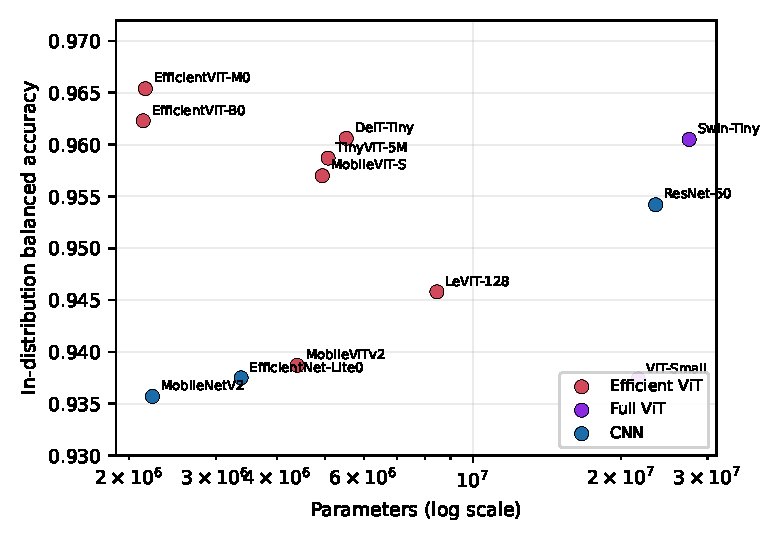
\includegraphics[width=0.82\textwidth]{figs/p1_fig1_params_vs_accuracy.pdf}
\caption{Parameters (log scale) vs.\ in-distribution balanced accuracy,
colored by architecture family. The two efficient-ViT models with the
fewest parameters (EfficientViT-M0/B0) are also the two most accurate.}
\label{fig:params-vs-acc}
\end{figure}

\subsection{Cross-dataset domain shift, escalating from 2 to 12 models}

\textbf{Stage 1 (DeiT-Tiny alone):} in distribution 0.9504 balanced
accuracy, Herlev (zero-shot) 0.7151, Mendeley LBC (zero-shot) 0.5230 -- a
model that looks excellent in distribution degrades to near-chance on the
more severe external dataset, with nothing in a standard pipeline able to
flag this.

\textbf{Stage 2 (adding EfficientViT-M0):} the \emph{better}
in-distribution model (0.9737 vs.\ DeiT-Tiny's 0.9504) is the
\emph{worse} model under both shifts (Herlev 0.6716 vs.\ 0.7151; Mendeley
LBC 0.4731 vs.\ 0.5230 -- the first model in this study to drop below the
0.50 chance floor). Two models this close in architecture family and
parameter count producing this reversal is a direct caution against using
in-distribution accuracy as a proxy for deployment robustness.

\textbf{Stage 3 (adding ResNet-50 and Swin-Tiny):}

\begin{table}[htbp]
\centering
\caption{One model per architecture family under cross-dataset shift.}
\label{tab:rq4-stage3}
\begin{tabular}{lrrr}
\toprule
Model (family) & SIPaKMeD & Herlev & Mendeley LBC \\
\midrule
EfficientViT-M0 (efficient ViT) & \textbf{0.9737} & 0.6716 & \textbf{0.4731} (below chance) \\
Swin-Tiny (full ViT) & 0.9590 & \textbf{0.7282} & 0.5192 \\
DeiT-Tiny (efficient ViT) & 0.9504 & 0.7151 & 0.5230 \\
ResNet-50 (CNN) & 0.9556 & 0.6838 & \textbf{0.6082} \\
\bottomrule
\end{tabular}
\end{table}

Not a clean CNN-vs-transformer split: on Herlev, both transformer models
beat ResNet-50. What holds across both shift datasets is narrower: the
single most parameter-efficient, best-in-distribution model
(EfficientViT-M0) is the worst performer under shift on both external
datasets, and the only one below chance on either.

\textbf{Stage 4 (all 12 models):}

\begin{table}[htbp]
\centering
\caption{Full 12-model cross-dataset shift evaluation, sorted by Mendeley LBC score.}
\label{tab:rq4-full}
\begin{tabular}{lrrr}
\toprule
Model (family, params) & SIPaKMeD & Herlev & Mendeley LBC \\
\midrule
EfficientNet-Lite0 (CNN, 3.38M) & 0.9455 & 0.5970 & \textbf{0.6674} \\
ResNet-50 (CNN, 23.5M) & 0.9556 & 0.6838 & 0.6082 \\
MobileViTv2 (eff.\ ViT, 4.39M) & 0.9638 & \textbf{0.7501} & 0.5418 \\
MobileNetV2 (CNN, 2.23M) & 0.9505 & 0.6919 & 0.5391 \\
DeiT-Tiny (eff.\ ViT, 5.5M) & 0.9504 & 0.7151 & 0.5230 \\
EfficientViT-B0 (eff.\ ViT, 2.14M) & 0.9738 & 0.6818 & 0.5217 \\
Swin-Tiny (full ViT, 27.5M) & 0.9590 & 0.7282 & 0.5192 \\
ViT-Small (full ViT, 21.7M) & 0.9573 & 0.7049 & 0.5084 \\
LeViT-128 (eff.\ ViT, 8.4M) & 0.9526 & 0.5777 & 0.4764 \\
EfficientViT-M0 (eff.\ ViT, 2.16M) & 0.9737 & 0.6716 & 0.4731 \\
TinyViT-5M (eff.\ ViT, 5.1M) & 0.9685 & \textbf{0.7327} & 0.4543 \\
MobileViT-S (eff.\ ViT, 4.94M) & 0.9520 & 0.7104 & \textbf{0.2927} (AUROC 0.215) \\
\bottomrule
\end{tabular}
\end{table}

A near-clean CNN-vs-transformer split emerges on Mendeley LBC, with one
exception: all three CNNs land at 0.539--0.667; eight of nine
transformer-family models land at 0.293--0.523; the ninth (MobileViTv2)
scores 0.5418, above the lowest CNN (0.5391) by 0.003 -- a gap
seed-variance testing (Section~5, Internal validity) shows is noise, not
a real difference. This split does not hold on Herlev, where transformer
models occupy both the best (MobileViTv2, TinyViT-5M) and weaker
(LeViT-128) positions.

MobileViT-S is a severe, singular outlier: its Mendeley LBC AUROC (0.215)
is not merely below chance but actively anti-correlated with ground
truth. Its direct successor, MobileViTv2, shows no such problem and is the
single strongest model in the entire registry on Herlev (0.7501) -- the
same architecture-family name spanning a catastrophic failure and a top
performer, ruling out architecture lineage as a predictor of shift
robustness as thoroughly as parameter count and in-distribution accuracy
already have been.

\begin{figure}[htbp]
\centering
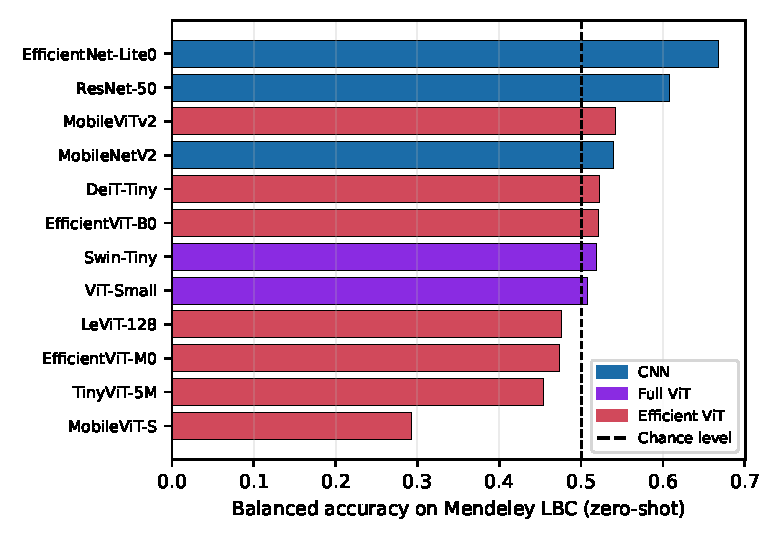
\includegraphics[width=0.82\textwidth]{figs/p1_fig2_mendeley_shift.pdf}
\caption{Balanced accuracy on Mendeley LBC (zero-shot), sorted, colored by
architecture family. All three CNNs cluster above chance; eight of nine
transformer-family models cluster at or below chance, with MobileViT-S
the sole catastrophic outlier.}
\label{fig:mendeley-shift}
\end{figure}

\textbf{Stage 5 (all 12 models, third independent shift dataset -- APCEM):}

\begin{table}[htbp]
\centering
\caption{Full 12-model evaluation on the third external shift dataset (APCEM), sorted by AUROC.}
\label{tab:rq1-apcem}
\begin{tabular}{lrrr}
\toprule
Model (family, params) & SIPaKMeD & APCEM bal.\ acc. & APCEM AUROC \\
\midrule
MobileNetV2 (CNN, 2.23M) & 0.9623 & \textbf{0.6158} & \textbf{0.6528} \\
EfficientNet-Lite0 (CNN, 3.38M) & 0.9309 & 0.5393 & 0.5701 \\
LeViT-128 (eff.\ ViT, 8.4M) & 0.9001 & 0.5263 & 0.5376 \\
Swin-Tiny (full ViT, 27.5M) & 0.9330 & 0.4724 & 0.3082 \\
EfficientViT-B0 (eff.\ ViT, 2.14M) & 0.9638 & 0.4481 & 0.3206 \\
DeiT-Tiny (eff.\ ViT, 5.5M) & 0.9589 & 0.4469 & 0.3799 \\
MobileViTv2 (eff.\ ViT, 4.39M) & 0.9570 & 0.4290 & 0.4120 \\
TinyViT-5M (eff.\ ViT, 5.1M) & 0.9670 & 0.4100 & 0.3681 \\
EfficientViT-M0 (eff.\ ViT, 2.16M) & 0.9621 & 0.3730 & 0.3407 \\
MobileViT-S (eff.\ ViT, 4.94M) & 0.9687 & 0.3621 & 0.3161 \\
ViT-Small (full ViT, 21.7M) & 0.9538 & 0.3444 & 0.2555 \\
ResNet-50 (CNN, 23.5M) & 0.9639 & \textbf{0.3339} & \textbf{0.2929} \\
\bottomrule
\end{tabular}
\end{table}

APCEM is a genuinely independent replication -- different acquisition
pipeline, institution, and label granularity from either Herlev or
Mendeley LBC -- and it does not merely confirm the earlier finding that
in-distribution accuracy fails to predict shift robustness (11 of 12
models land at or below the 0.50 chance floor for balanced accuracy on
APCEM, several with AUROC well below 0.35), it overturns the one pattern
that had looked stable across Stages 3--4: that CNN-family models cluster
above chance while transformer-family models cluster at or below it. Here
the CNN family alone spans the single best-performing model in the entire
registry (MobileNetV2, 0.6158 balanced accuracy, the only model of the 12
to clear chance meaningfully) and one of the single worst
(ResNet-50, AUROC 0.2929, second-lowest of all 12) -- the same family that
was the more robust one, on average, on Mendeley LBC. DeiT-Tiny and
EfficientViT-M0, the two models directly compared since Stage 2, again
replicate their earlier ranking (DeiT-Tiny 0.4469 vs.\ EfficientViT-M0
0.3730), with EfficientViT-M0 again the weaker model under shift despite
again being the stronger in-distribution model on this run (0.9621 vs.\
0.9589) -- the same reversal, now observed on a third, independently
sourced dataset.

\begin{figure}[htbp]
\centering
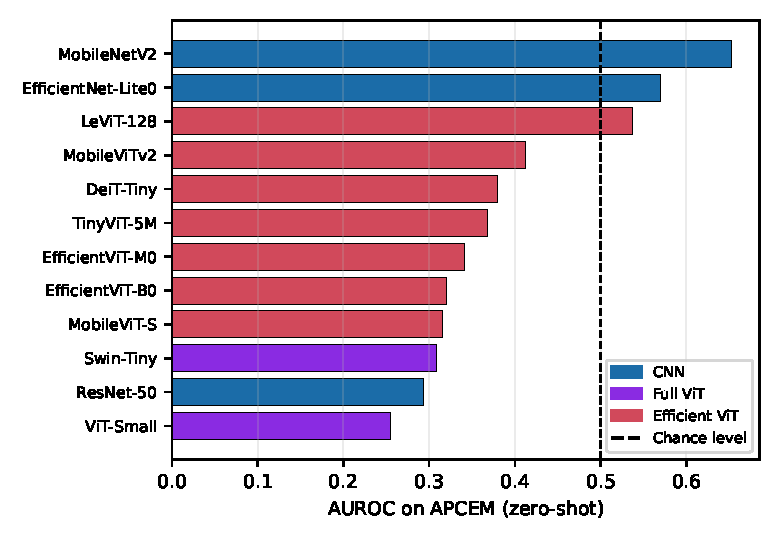
\includegraphics[width=0.82\textwidth]{figs/p1_fig3_apcem_shift.pdf}
\caption{AUROC on APCEM (zero-shot), sorted, colored by architecture
family. Unlike Mendeley LBC, the CNN family spans both the single best
(MobileNetV2) and one of the single worst (ResNet-50) models in the
registry -- no family-level pattern survives this third dataset.}
\label{fig:apcem-shift}
\end{figure}

\section{Discussion}

Four findings, read together, argue against four different intuitive
heuristics for selecting a deployment backbone from an in-distribution
benchmark alone. First, ``smaller is worse'' is directly falsified in
distribution (Section~4.1). Second, ``the in-distribution winner is the
safe choice'' is directly falsified under shift (Section~4.2, Stage~2):
the model with the best in-distribution accuracy in the entire study is
the worst-performing model under both Herlev and Mendeley LBC shift,
dropping below the chance floor on one, and it replicates this same
reversal on APCEM (Stage~5). Third, ``architecture family/lineage
predicts robustness'' is falsified by MobileViT-S and MobileViTv2 sharing
a name and a lineage while producing a catastrophic failure and a top
performance, respectively, on the same evaluation. Fourth, and only
visible once a third, independently sourced shift dataset is added:
``CNNs are the robust family'' -- a pattern that looked genuinely stable
across Stages 3--4, where all three CNNs outperformed eight of nine
transformer models on Mendeley LBC -- is directly falsified on APCEM,
where the CNN family spans both the single best-performing model in the
entire registry (MobileNetV2) and one of the single worst (ResNet-50).
That reversal is the paper's sharpest methodological warning: even a
robustness pattern that survives two independent shift datasets is not
guaranteed to survive a third, so ``tested under two external shifts''
should not be read as license to stop testing. The practical implication
is direct: a deployment decision based on an in-distribution leaderboard,
however carefully measured, cannot be assumed to transfer to real
cross-institution conditions, and no static property measured here --
including which architecture family fared best on the shift datasets
tested so far -- substitutes for actually testing under the specific
shift a deployment will face. This motivates the uncertainty-quantification
question our companion paper asks: since no backbone choice alone is
safe, can a model's own confidence signal at least correctly flag when it
has entered a regime where its predictions should not be trusted?

\section{Threats to Validity}

\textbf{Internal validity.} Each headline model was trained once (seed
13); we measured seed-to-seed variance directly for this paper's two
closest-ranked pairs rather than leaving it as a caveat, at two more
seeds (17, 29). On Mendeley LBC, MobileViTv2's 0.003 edge over
MobileNetV2 (0.5418 vs.\ 0.5391, Table~3) does \emph{not} survive:
MobileNetV2 ranges 0.493--0.604 and MobileViTv2 ranges 0.494--0.623
across the three seeds, the ranges overlap almost completely, and the
ranking flips under seed 17. That gap is sampling noise, not a real
difference. On APCEM, EfficientViT-B0's 0.001 edge over DeiT-Tiny
(0.4481 vs.\ 0.4469, Table~4) \emph{does} survive: EfficientViT-B0 ranges
0.421--0.448, DeiT-Tiny ranges 0.367--0.447, EfficientViT-B0 wins all
three seeds, and its margin widens (to 0.027, then 0.067) rather than
shrinking. The same close-call caveat produced opposite outcomes once
tested -- a direct caution against assuming either direction from a
single seed. No trained-weight checkpoints persist across sessions, so
results could not be re-verified from the original weights without full
retraining; the reported numbers are the direct, unedited output of the
released training and evaluation code, which mitigates but does not
eliminate this threat.

We extended this check from the 2 closest-ranked pairs to all 12 models,
at the same 2 extra seeds, evaluated zero-shot on all three external
datasets from a single checkpoint per model per seed
(\texttt{docs/rq1\_seedcheck\_full\_results.md}). Two further findings
sharpen, rather than soften, the paper's central claim. First, the
``near-clean'' CNN-vs-transformer split reported for Mendeley LBC
(Section~4.2, Stage~4) is itself a property of seed 13, not of the
dataset: only 1 of 9 transformer-family models exceeds the weakest CNN at
seed 13 (by 0.003, already flagged above as noise), but 3 of 9 do at seed
17 and 4 of 9 do at seed 29, by margins up to 0.11 -- an order of
magnitude past the single close call this section already discounts.
Second, EfficientViT-M0 -- this paper's running illustration of ``the
in-distribution winner is the shift-robustness loser''
(Section~4.1, Conclusion) -- does not reliably occupy either role: it is
the (near-)in-distribution winner and one of the two worst shift
performers on Herlev and Mendeley LBC at seed 13, but at seed 29 it is the
outright in-distribution winner \emph{and} mid-pack under shift on both
datasets (rank 4--5 of 12), and at seed 17 it is not even the
in-distribution winner (rank 10 of 12). The general claim this example
illustrates -- that no static property predicts shift robustness -- is
unaffected, and if anything reinforced (a poster-child example that
itself varies by seed is one more demonstration of that unreliability);
what changes is that this specific model should be read as a
seed-13-specific illustration rather than a reproducible property of
EfficientViT-M0. Not every seed-checked finding is this fragile: Herlev's
inverse pattern (most transformer models outscoring the CNNs) and
MobileNetV2's status as the strongest model on APCEM both replicate
cleanly across all three seeds.

\textbf{External validity.} All four datasets are drawn from a small
number of source institutions (SIPaKMeD, Herlev, Mendeley LBC, and APCEM
together represent four geographic/clinical sources), and generalization
to other scanners, staining protocols, or populations beyond these four is
not established. The three shift conditions tested (Herlev, Mendeley LBC,
APCEM) are real cross-institution shifts, not a systematic sweep across
shift types (e.g., scanner resolution, stain intensity, patient
demographics varied independently), so the finding that no static model
property predicts shift robustness is demonstrated for these three shifts
specifically, not proven for shift in general. The APCEM result itself is
direct evidence for why this caveat matters in practice, not just in
principle: the CNN-family robustness pattern that held across the first
two shift datasets did not survive the third, so a reader should not
assume the specific findings reported here (e.g., which individual model
is most robust) transfer to a fourth, untested shift condition either --
only the higher-level conclusion, that no static property reliably
predicts shift robustness, is expected to generalize.

\textbf{Construct validity.} Balanced accuracy, macro F1, and AUROC are
standard, well-understood metrics for imbalanced multi-class
classification, reducing the risk that the efficiency or robustness
claims are artifacts of an unusual metric choice. Measured CPU/GPU
latency (Table~1) is a single-run, single-batch-size figure per model and
is not the focus of this paper's central claims (which concern accuracy
and robustness), so its precision is secondary to the accuracy/robustness
findings the paper's contributions rest on.

\section{Limitations}

Three external datasets, all drawn from a small number of source
institutions; the shift conditions tested here are real but not
exhaustive of the shift a deployed system might encounter, and the
architecture-family pattern found stable across the first two shift
datasets (Section~4.2, Stages 3--4) did not survive the third (Stage~5),
so any single-dataset robustness ranking reported here should be read as
specific to that dataset rather than as a general robustness ordering. Each
headline result is a single train/val/calibration/test split (seed 13);
results are not averaged over multiple seeds, though seed-to-seed variance
was measured directly (Threats to Validity, Internal validity) across all
12 models at 2 further seeds rather than left unmeasured. That check found
some single-model and single-dataset claims are seed-specific rather than
general (the Mendeley LBC CNN-vs-transformer split, and EfficientViT-M0
specifically as the in-distribution-winner-becomes-shift-loser example),
so individual rows and close-ranked comparisons in these tables should be
read with that caution; the paper's higher-level conclusions do not rest
on any single seed-fragile comparison. No trained-weight checkpoints
persist; reproducing any single row of these tables means retraining from
scratch.

\section{Conclusion}

Twelve models across three architecture families show that, on this
cervical cytology classification task, parameter-efficient vision
transformers do not trade accuracy for efficiency -- the smallest models
in the registry are also the most accurate in distribution. But that same
efficiency-and-accuracy leaderboard actively misleads about deployment
robustness: the overall in-distribution winner is the worst-performing
model under real cross-dataset shift on two of the three external datasets
tested, and no static property we measured reliably predicts which model
fails safely. A third, independently sourced shift dataset (APCEM)
sharpens this warning rather than merely repeating it: even the one
pattern that survived the first two shift datasets -- that CNN-family
models are, on average, more robust than transformer-family models --
collapses on the third, where the CNN family contains both the single
best- and one of the single worst-performing models in the entire
registry. Robustness must be measured directly, under the real shift a
deployment will actually face, and cannot be inferred from an
in-distribution benchmark however thorough, nor safely generalized from a
robustness pattern observed on only one or two external datasets.

\begin{thebibliography}{99}

\bibitem{plissiti2018sipakmed}
Plissiti, M.E., Dimitrakopoulos, P., Sfikas, G., Nikou, C., Krikoni, O.,
Charchanti, A.: SIPAKMED: A new dataset for feature and image based
classification of normal and pathological cervical cells in Pap smear
images. In: 2018 IEEE International Conference on Image Processing
(ICIP), pp.\ 3144--3148 (2018)

\bibitem{he2016resnet}
He, K., Zhang, X., Ren, S., Sun, J.: Deep residual learning for image
recognition. In: CVPR (2016)

\bibitem{sandler2018mobilenetv2}
Sandler, M., Howard, A., Zhu, M., Zhmoginov, A., Chen, L.C.: MobileNetV2:
Inverted residuals and linear bottlenecks. In: CVPR (2018)

\bibitem{tan2019efficientnet}
Tan, M., Le, Q.: EfficientNet: Rethinking model scaling for convolutional
neural networks. In: ICML (2019)

\bibitem{dosovitskiy2021vit}
Dosovitskiy, A., et al.: An image is worth 16x16 words: Transformers for
image recognition at scale. In: ICLR (2021)

\bibitem{liu2021swin}
Liu, Z., Lin, Y., Cao, Y., Hu, H., Wei, Y., Zhang, Z., Lin, S., Guo, B.:
Swin Transformer: Hierarchical vision transformer using shifted windows.
In: ICCV (2021)

\bibitem{touvron2021deit}
Touvron, H., Cord, M., Douze, M., Massa, F., Sablayrolles, A., J\'egou,
H.: Training data-efficient image transformers \& distillation through
attention. In: ICML (2021)

\bibitem{graham2021levit}
Graham, B., El-Nouby, A., Touvron, H., Stock, P., Joulin, A., J\'egou, H.,
Douze, M.: LeViT: a vision transformer in ConvNet's clothing for faster
inference. In: ICCV (2021)

\bibitem{wu2022tinyvit}
Wu, K., et al.: TinyViT: Fast pretraining distillation for small vision
transformers. In: ECCV (2022)

\bibitem{mehta2022mobilevit}
Mehta, S., Rastegari, M.: MobileViT: Light-weight, general-purpose, and
mobile-friendly vision transformer. In: ICLR (2022)

\bibitem{mehta2022mobilevitv2}
Mehta, S., Rastegari, M.: Separable self-attention for mobile vision
transformers. arXiv preprint (2022)

\bibitem{cai2023efficientvit}
Cai, H., Li, J., Hu, M., Gan, C., Han, S.: EfficientViT: Multi-scale
linear attention for high-resolution dense prediction. In: ICCV (2023)

\bibitem{liu2023efficientvit}
Liu, X., Peng, H., Zheng, N., Yang, Y., Hu, H., Yuan, Y.: EfficientViT:
Memory efficient vision transformer with cascaded group attention. In:
CVPR (2023)

\bibitem{jantzen2005herlev}
Jantzen, J., Norup, J., Dounias, G., Bjerregaard, B.: Pap-smear benchmark
data for pattern classification. In: Proceedings of Nature Inspired Smart
Information Systems (NiSIS), pp.\ 1--9 (2005)

\bibitem{hussain2020mendeley}
Hussain, E., Mahanta, L.B., Borah, H., Das, C.R.: Liquid based-cytology
Pap smear dataset for automated multi-class diagnosis of pre-cancerous
and cervical cancer lesions. Data in Brief 30, 105589 (2020)

\bibitem{mohiuddin2025}
Mohiuddin, A.B., Rahman, M.M., et al.: Accelerated and accurate cervical
cancer diagnosis using a novel stacking ensemble method with explainable
AI. In: International Conference on Quantum Photonics, Artificial
Intelligence (2025)

\bibitem{aswini2026apcem}
Aswini, H.: APCEM-Enhanced Cervical Cytology Image Dataset (Version 2)
[Data set]. Mendeley Data (2026). \url{https://doi.org/10.17632/snzb5g6ddy.2}

\end{thebibliography}
\end{document}
